% Kopfzeile beim Kapitelanfang:
\fancypagestyle{plain}{
%Kopfzeile links bzw. innen
\fancyhead[L]{\Large Vorlesung 17 (09.12.2013)}
%Kopfzeile rechts bzw. außen
\fancyhead[R]{}}
%Kopfzeile links bzw. innen
\fancyhead[L]{\Large Vorlesung 17 (09.12.2013)}
%Kopfzeile rechts bzw. außen
\fancyhead[R]{}
% **************************************************
\section{Definition: Stetigkeit komplexer Funktionen}\label{9.7}
Sei $D \subseteq \C, f: D \to \C$ heißt stetig in $z_0 \in D :\Lra$
$$\forall \eps > 0 \exists \delta > 0: |f(z)-f(z_0)| < \eps \forall z \in D: |z-z_0| < \delta$$
\begin{tikzpicture}
\draw[->] (-1,0)--(3,0);
\draw[->] (0,-1)--(0,3);
\draw (-0.5,3) circle (0.3) node {$\C$};
\draw[pattern=north east lines] (1,1) circle (0.5);
\draw (1,1)--(2,1.25) node[right] {$\delta$};
\draw (1.5,0.5) node {$z_0$};
\draw (0.75,0.75) ellipse (2 and 1.5);
\draw (-0.5,0.5) node {$D$};
\end{tikzpicture} \ $\underset{f}{\to}$ \ 
\begin{tikzpicture}
\draw[->] (-1,0)--(3,0);
\draw[->] (0,-1)--(0,3);
\draw (-0.5,3) circle (0.3) node {$\C$};
\draw[pattern=north east lines] (1,1) circle (0.5);
\draw (1,1)--(2,1.25) node[right] {$\eps$};
\draw (1.75,0.5) node {$f(z_0)$};
\end{tikzpicture}\nl
$f$ stetig auf $D :\Lra f$ stetig in jedem $z_0 \in D$

\section{Folgenkriterium für komplexe Funktionen}\label{9.8}
$f: D \to \C$ ist stetig in $z_0 \in D \Lra$
$$\forall (z_n) \subseteq D, z_n \to z_0: f(z_n) \to f(z_0)$$

\subsection*{Beweis}
Wörtlich wie für $\R$ (\ref{9.2})

\section{Beispiele}\label{9.9}
\en{
\item Jedes Polynom $p(z) = a_k z^k + \ldots + a_1 z + a_0 \in \Pow_\C$ ist stetig auf $\C$, denn:\\
$z_n \to z_0 \in \C \underset{\text{Regeln für Grenzwerte}}{\Ra} p(z_n) \to p(z_0) \underset{\text{Folgenk. \ref{9.8}}}{\Ra} p$ stetig in $z_0$
\item $exp: \C \to \C, z \mto e^z$ ist stetig auf $\C$\\
Beweis: Wörtlich wie Satz \ref{9.5} (reeller Fall)
}
Die Regeln \ref{9.3} sowie \ref{9.6} (Summen, Produkte, Quotienten, Komposition) gelten entsprechend auch für komplexe Funktionen.

\section{Korollar}\label{9.10}
$cos: \R \to \R$ und $sin: \R \to \R$ sind stetig auf $\R$.

\subsection*{Beweis (für $cos$ und $sin$ analog)}
Sei $x_0 \in \R, (x_n) \subseteq \R: x_n \to x_0$\\
$cos \ x = \RE(e^{ix})$\\
$x_n \to x_0 \Ra i x_n \to i x_0$ (in $\C$) $\underset{exp \text{ stetig}}{\Ra} e^{i x_n} \to e^{i x_0} \Ra cos(x_n) = \RE(e^{i x_n}) \underset{\text{\ref{6.16}}}{\to} \RE(e^{i x_0}) = cos(x_0)$\\
$\Ra cos$ ist stetig in $x_0$. \qed

\newpage

\phantomsection
\addcontentsline{toc}{section}{Grenzwerte bei Funktionen}
\section*{Grenzwerte bei Funktionen}
Beispiel: $f(x) = \frac{e^x-1}{x}, D = \R \setminus \{0\}$\\
Wie sieht $f$ nahe $0$ aus?\nl
Betrachte $f(x_n)$ für $(x_n) \subseteq \R \setminus \{0\}$ mit $x_n \to 0$

\section{Definition}\label{9.11}
Sei $D \subseteq \R, f: D \to \R$ Funktion und \underline{$x_0 \in \R$}.\\
Man sagt: $f$ konvergiert für $x \to x_0$ gegen $c \in \R \cup \{\pm \infty\} :\Lra \forall (x_n) \subseteq D, x_n \to x_0: f(x_n) \to c$\nl
Dabei wird vorausgesetzt, dass es mindestens eine Folge $(x_n) \subseteq D$ gibt mit $x_n \to x$.\\
$c$: \underline{Grenzwert} von $f$ in $x_0$\\
Schreibweise: $\lim_{x \to x_0} f(x) = c$ oder $f(x) \to c$ für $x \to x_0$\nl
\fbox{\begin{tikzpicture}
\draw (0,0)--(2,0);
\draw (2,0) node {$|$};
\draw (1,-0.3) node {$D$};
\draw (1,-0.8) node {$\nexists(x_n)$};
\draw (3.5,0) node{$\cdot$} node[below] {$x_0 \notin D$};
\end{tikzpicture}} \ 
\fbox{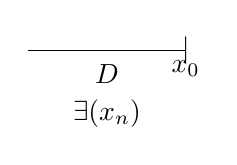
\begin{tikzpicture}
\draw (0,0)--(2,0);
\draw (2,0) node {$|$} node[below] {$x_0$};
\draw (1,-0.3) node {$D$};
\draw (1,-0.8) node {$\exists(x_n)$};
\end{tikzpicture}} \ 
\fbox{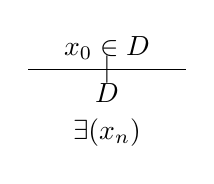
\begin{tikzpicture}
\draw (0,0)--(2,0);
\draw (1,0) node {$|$} node[above] {$x_0 \in D$};
\draw (1,-0.3) node {$D$};
\draw (1,-0.8) node {$\exists(x_n)$};
\end{tikzpicture}}\nl
Beachte:
\en{
\item \underline{Falls $x_0 \in D$} $\Ra x_n=x_0$ wählbar $\forall n$ (konstante Folge).\\
Also: $\lim_{x \to x_0} f(x) = 0 \Ra c = f(x_0)$\\
Und: $\lim_{x \to x_0} f(x) = f(x_0) \Lra f$ stetig in $x_0$ (nach Folgenkriterium \ref{9.2}).
\item \underline{Falls $c \in \{\pm \infty\}$} ist $\lim_{x \to x_0} f(x) = c$ uneigentlicher Grenzwert
}
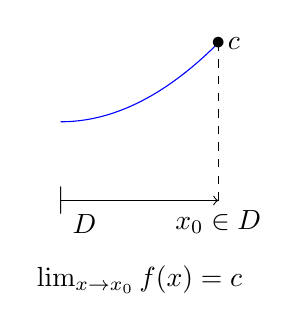
\begin{tikzpicture}
\draw[->] (0,0)--(2,0) node[below] {$x_0 \in D$};
\draw (0,0) node {$|$};
\draw (0.3,-0.3) node {$D$};
\draw (1,-1) node {$\lim_{x \to x_0} f(x)=c$};
\draw[color=blue,domain=0:2] plot (\x, {0.25*(\x^2)+1});
\draw (2,2) node {$\bullet$} node[right] {$c$};
\draw[dashed] (2,0)--(2,2);
\end{tikzpicture} \ 
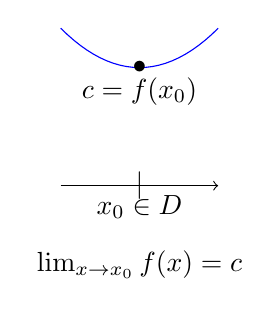
\begin{tikzpicture}
\draw[->] (-1,0)--(1,0);
\draw (0,0) node {$|$} node[below] {$x_0 \in D$};
\draw[color=blue,domain=-1:1] plot (\x, {0.5*abs(\x^2)+1.5});
\draw (0,1.5) node {$\bullet$} node[below] {$c=f(x_0)$};
\draw (0,-1) node {$\lim_{x \to x_0} f(x)=c$};
\end{tikzpicture} \ 
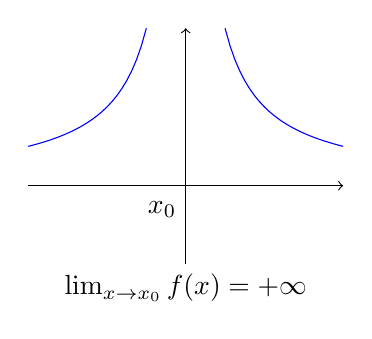
\begin{tikzpicture}
\draw[->] (-2,0)--(2,0);
\draw[->] (0,-1)--(0,2);
\draw (-0.3,-0.3) node {$x_0$};
\draw[color=blue,domain=0.5:2] plot (\x, {1/\x});
\draw[color=blue,domain=-2:-0.5] plot (\x, {abs(1/\x)});
\draw (0,-1.3) node{$\lim_{x \to x_0} f(x) = +\infty$};
\end{tikzpicture}

\subsection*{Beachte}
\underline{Falls $x_0 \notin D$}: Dann $\lim_{x \to x_0} f(x) = c \Lra$ die Fortsetzung
$$\tilde{f}(x) := \left\{ \begin{array}{l} f(x), x \in D \\ c, x = x_0 \end{array} \right., \tilde{f}: D \cup \{x_0\} \to \R$$
ist stetig in $x_0$

\section{Korollar}\label{9.12}
$\lim_{x \to x_0} f(x) = c \in \R \Lra$
$$\forall \eps > 0 \exists \delta > 0: |f(x)-c| < \eps \forall x \in D: |x-x_0| < \delta$$

\newpage

\section{Einseitige Grenzwerte}\label{9.13}
Gegeben: Funktion $f: D \to \R$, $x_0 \in \R$\nl
$c \in \R \cup \{\pm\infty\}$ heißt rechtsseitiger Grenzwert von $f$ in $x_0 :\Lra$\\
$\lim_{\{x \in D: x > x_0\}, x \to x_0} f(x) = c$\nl
Schreibweise: $\lim_{x \downarrow x_0} f(x) = c$\\
Analog: Linksseitiger Grenzwert $\lim_{x \uparrow x_0} f(x) = \lim_{\{x \in D: x < x_0\}, x \to x_0} f(x)$\nl
\begin{tikzpicture}
\draw (-3,0)--(3,0);
\draw (0,0) node{$|$} node[below] {$x_0$};
\draw[color=blue,domain=-2.5:0] plot (\x, {0.25*(-(-\x^2))+1});
\draw[color=blue,domain=0:2.5] plot (\x, {0.25*(\x-2.5)^2+0.4375});
\draw[dashed] (0,0)--(0,2);
\draw (0,1) node {$\bullet$} node[right] {$c_1$};
\draw (0,2) node {$\bullet$} node[left] {$c_2$};
\end{tikzpicture}

\section{Beispiele}\label{9.14}
\en{
\item $f(x)=\frac{x^2-1}{x-1} \Ra \lim_{x \to 1} f(x) = \lim_{x \to 1} \underbrace{(x+1)}_{\text{stetig in } x=1} = 2$
\item Heaviside-Funktion: $H(x) = \left\{\begin{array}{l} 1, x \ge 0 \\ 0, x < 0 \end{array} \right.$\\
\begin{tikzpicture}
\draw[->] (-2,0)--(2,0);
\draw[->] (0,-0.5)--(0,2);
\draw[thick,color=blue] (-2,0)--(0,0);
\draw (-0.2,-0.2) node {$0$};
\draw[thick,color=blue] (0,1)--(2,1);
\draw (-0.2,1) node {$1$};
\draw[color=blue] (0,0) node {$\bullet$};
\draw[color=blue] (0,1) node {$\bullet$};
\draw[dashed] (-2,0.5)--(2,0.5);
\draw[dashed] (-2,1.5)--(2,1.5);
\draw [decoration={brace,mirror,raise=0.5cm},decorate] (1.6,0.5)--(1.6,1);
\draw (2.4,0.75) node {$\frac{1}{2}$};
\end{tikzpicture}\nl
$\lim_{x \uparrow 0} H(x) = 0$ (denn: $(x_n) \subseteq \R, x_n < 0, x_n \to 0 \Ra H(x_n) = 0$)\\
$\lim_{x \downarrow 0} H(x) = 1 = H(0)$\\
$\lim_{x \to 0} H(x)$ existiert nicht
\item $f(x) = \frac{1}{x}$ auf $\R \setminus \{0\}$\nl
\begin{tikzpicture}
\draw[->] (-2,0)--(2,0);
\draw[->] (0,-2)--(0,2);
\draw (-0.2,-0.2) node {$0$};
\draw[color=blue,domain=-2:-0.5] plot (\x, {1/\x});
\draw[color=blue,domain=0.5:2] plot (\x, {1/\x});
\end{tikzpicture}\nl
$\lim_{x \downarrow 0} f(x) = + \infty$, denn:\\
$x_n \downarrow 0 \Ra \frac{1}{x_n} \to + \infty$\\
$\lim_{x \uparrow 0} f(x) = - \infty$\nl
Dagegen: $f(x)=\frac{1}{x^2}$, $\lim_{x \to 0} \frac{1}{x^2} = + \infty$\nl
\begin{tikzpicture}
\draw[->] (-2,0)--(2,0);
\draw[->] (0,-0.5)--(0,2);
\draw (-0.2,-0.2) node {$0$};
\draw[color=blue,domain=-2:-0.707106781] plot (\x, {1/abs(\x^2)});
\draw[color=blue,domain=0.707106781:2] plot (\x, {1/abs(\x^2)});
\end{tikzpicture}
\item \fbox{$\lim_{x \to 0} \frac{e^x-1}{x} = 1$}\\
$e^x = 1 + x + \frac{x^2}{2} + \ldots$\\
$\frac{e^x-1}{x} = 1 + \frac{x}{2} + \ldots$\nl
\underline{Beweis}: $|e^x-1-x| \le |x^2|$ für $|x| \le 1$ (Restgliedabschätzung, \ref{8.12})\\
$\Ra \left|\frac{e^x-1}{x} -1\right| \le |x|$ für $|x| \le 1$, $x \neq 0$\\
Sei $(x_n) \subseteq \R \setminus \{0\}$ Folge mit $x_n \to 0 \Ra$ für $n$ groß genug\\
$\left|\frac{e^{x_n}-1}{x_n} - 1\right| \le |x_n| \underset{n \to \infty}{\to} 0 \Ra \frac{e^{x_n} -1}{x_n} \to 1$\nl
\underline{Alternativer Beweis} mit Korollar \ref{9.12} ($\eps$-$\delta$-Bed.)\\
Sei $\eps > 0$ gegeben. (*) $\Ra \left|\frac{e^x -1}{x} - 1\right| < \eps$ für alle $x \neq 0$ mit $|x| < \eps$ (o.E. $\eps < 1$)\\
$\underset{\text{\ref{9.12}}}{\Ra}$ Behauptung \qed
}

\section{\texorpdfstring{Grenzwerte für $x \to \pm \infty$}{Grenzwerte für x gegen +- Unendlich}}\label{9.15}
Gegeben: Funktion $f: D \to \R, D \subseteq \R$ nach oben unbeschränkt.\\
$\lim_{x \to +\infty} f(x) = c \in \R \cup \{\pm\infty\} :\Lra$\\
$\forall (x_n) \subseteq D$ mit $x_n \to +\infty$ gilt $f(x_n) \to c$\nl
\begin{tikzpicture}
\draw[->] (-1,0)--(3,0);
\draw[->] (0,-1)--(0,3);
\draw[color=blue,domain=-1:3] plot (\x, {(exp(-(\x)))+0.5});
\draw[dashed] (-1,0.5)--(3,0.5);
\draw (-0.5,0.25) node {$c$};
\end{tikzpicture} \ 
\begin{tikzpicture}
\draw[->] (-2,0)--(3,0);
\draw[->] (0,-1)--(0,3);
\draw[color=blue,domain=-2:0] plot (\x, {0.25*sin(deg(10*\x))+1});
\draw[color=blue,domain=0:2] plot (\x, {0.5*\x^2+1});
\draw (1.5,-0.5) node {$\lim_{x \to \infty} f(x) = +\infty$};
\end{tikzpicture}\nl
Analog: $\lim_{x \to -\infty} f(x)$, falls $D$ nach unten unbeschränkt.

\subsection*{Beispiel}
$\lim_{x \to +\infty} \frac{1}{x} = 0 = \lim_{x \to -\infty} \frac{1}{x}$\\
(denn: $x_n \to \pm \infty \Ra \frac{1}{x_n} \to 0$)

\newpage

\section{Regeln für Grenzwerte von Funktionen}\label{9.16}
Ergeben sich aus den Regeln für Folgen-Grenzwerte (ab \ref{5.2}), z.B.:\\
$f,g: D \to \R$ mit $f(x) \to a, g(x) \to b$ für $x \to x_0 \in \R \cup \{\pm\infty\}; a,b \in \R$ $\Ra$
\en{
\item $f(x) \underset{\cdot}{+} g(x) \to a \underset{\cdot}{+} b$ für $x \to x_0$,\\
$\frac{f(x)}{g(x)} \to \frac{a}{b}$ sofern $b \neq 0$
\item $f \le g$ auf $D \Ra a \le b$
}
Ferner: $f(x) \to \pm\infty$ für $x \to x_0 \Ra \frac{1}{f(x)} \to 0$ für $x \to x_0$

\section{Beispiele}\label{9.17}
\en{
\item $n \in \N_0 \Ra$ \fbox{$\lim_{x \to +\infty} \frac{e^x}{x^n} = +\infty$} (*)\nl
\begin{tikzpicture} [domain=-3:3]
\draw[->] (-3,0)--(3,0) node[right] {$x$};
\draw[->] (0,-0.5)--(0,3) node[above] {$f(x)$};
\draw[blue, domain=-3:1.2] plot (\x, {exp(\x)});
\draw[dashed] (1,0)--(1,2.7182818);
\draw[dashed] (0,2.7182818)--(1,2.7182818);
\draw (0,2.7182818) node{$-$} [left] node{$e$};
\draw (0,1) node{$-$} [left] node{$1$};
\draw (-0.3,-0.3) node{$0$};
\draw (1,0) node{$|$} [below] node{$1$};
\end{tikzpicture}\nl
Das heißt: $e^x$ wächst für $x \to +\infty$ schneller als jede Potenz von $x$.\\
\underline{Ferner}: $\lim_{x \to -\infty} x^n e^x \underset{y=-x}{=} \lim_{y \to +\infty} (-1)^n \frac{y^n}{e^y} \underset{\text{(*)}}{=} 0$\nl
\underline{Beweis von (*)}: $x > 0 \Ra e^x = \sum_{k=0}^\infty \frac{x^k}{k!} > \frac{x^{n+1}}{(n+1)!} \Ra \frac{e^x}{x^n} > \frac{x}{(n+1)!} \underset{x \to +\infty}{\to} +\infty$\\
$\Ra \frac{e^x}{x^n} \to +\infty$ \qed
\item \fbox{$\lim_{x \to 0} \frac{sin \ x}{x} = 1$} \ $sin \ x = x - \frac{x^3}{3!} \pm \ldots$\nl
\underline{Beweis}: Einschließungslemma (\ref{8.20}): $0 < x \le 2 \Ra 1 - \frac{x^2}{3} \le \frac{sin \ x}{x} \le 1$ ($\square$)\\
$f(x) = \frac{sin \ x}{x}$ ist gerade in $x$, d.h. $f(-x)=f(x)$\\
$\Ra$ ($\square$) gilt $\forall |x| \le 2, x \neq 0$\\
$\lim_{x \to 0} \left(1 - \frac{x^2}{6}\right) = 1 \underset{\text{\ref{5.8}}}{\Ra} \lim_{x \to 0} \frac{sin \ x}{x} = 1$
}